\documentclass[11pt,a4paper]{article}

%========== PACKAGES ==========%

\usepackage{a4wide} 			% save some rainforests
\usepackage{amsmath,amssymb}	% for mathematical notation
\usepackage[english]{babel}		% language definition
\usepackage{color}				% to make syntax pretty
\usepackage{enumerate}			% roman enumeration
\usepackage{fancyref}			% fancy references
\usepackage{float}				% for precise placement
\usepackage{graphicx}			% importing graphics
\usepackage{listings}			% code listings
\usepackage[utf8]{inputenc} 	% can we has UTF-8, plox
\usepackage{multicol} 			% for column layout
\usepackage{tikz} 				% pretty drawings

\usetikzlibrary{automata,arrows,positioning}	% make things easier

%========== DEFINITIONS ==========%

\definecolor{comment}{rgb}		{0.38, 0.62, 0.38}
\definecolor{keyword}{rgb}		{0.10, 0.10, 0.81}
\definecolor{identifier}{rgb}	{0.00, 0.00, 0.00}
\definecolor{string}{rgb}		{0.50, 0.50, 0.50}

\let\imp\to

%========== SETTINGS ==========%

\lstset
{
	% general settings
	numbers=left,
	frame=single,
	basicstyle=\footnotesize\ttfamily,
	tabsize=2,
	% syntax highlighting
	commentstyle=\color{comment},
	keywordstyle=\color{keyword},
	identifierstyle=\color{identifier},
	stringstyle=\color{string},
}

%========== DECLARATIONS ==========%

\title
{
	{\large Individual Assignment 3}\\
	Compilers
}

\author
{
	Casper B. Hansen\\
	Department of Computer Science\\
	University of Copenhagen\\
	{\tt fvx507@alumni.ku.dk}
}

%========== DOCUMENT ==========%

\begin{document}

\clearpage
\maketitle

\section{Exercise 1}
% Tests your understanding of parameter-passing conventions.
While the C language normally uses a call-by-value, there are other
conventions for passing parameters to functions, see corresponding slides in
Interpretation lecture notes.

Consider the C-like-syntax program below:
\lstinputlisting[language=C]{exercise-1.c}
In the following, what is printed if the calling conventions are used. Explain
briefly why.\footnote{These results were double-checked using a C++ program,
see attached program source {\tt call-by.cpp}.}
\begin{multicols}{3}

\subsection*{a \mdseries Call-by-value}
Using the call-by-value the function {\tt f} operates on copies.
\begin{lstlisting}[numbers=none]
	22
	5
	2
\end{lstlisting}
As we can see from the output, $x$ and $y$ stay unchanged.

\vfill\columnbreak

\subsection*{b \mdseries Call-by-reference}
The variables passed to the function are now references.
\begin{lstlisting}[numbers=none]
	33
	14
	5
\end{lstlisting}
This is why $x$ and $y$ are now different from when they were passed to the
function.

\vfill\columnbreak

\subsection*{c \mdseries Call-by-value-result}
Depending on the order we update the references.
\vspace{-0.23in}
\begin{multicols}{2}
\begin{lstlisting}[numbers=none]
	22
	12
	3
\end{lstlisting}
\vfill\columnbreak
\begin{lstlisting}[numbers=none]
	22
	7
	3
\end{lstlisting}
\vfill
\end{multicols}
\vspace{-0.21in}
\noindent This may have significance in multithreaded execution of programs.
\vfill
\end{multicols}

\newpage
\section{Exercise 2}
% Tests your understanding of dynamic/static scoping (see corresponding from
% Interpretation lecture notes).
Consider the C-like-syntax program:
\lstinputlisting[language=C]{exercise-2.c}
Exercises (a) and (b) were tested using a C++ program. See attached source
code in {\tt scoping.cpp} --- for (b) since C++ uses static scoping the way it
does it isn't faithful to dynamic scoping, but does simulate the effect.

\subsection*{a \mdseries With static  scoping, what would `f(4)' and `f(7)'
print, respectively? Explain briefly why.}
\begin{multicols}{2}

\noindent {\bf Output of {\tt f(4)}}
\begin{lstlisting}[language=C,numbers=none]
	5
\end{lstlisting}
The {\tt if} is matched and calls {\tt g}, which prints $5$ because the global
$x$ is bound to {\tt g}.

\vfill\columnbreak

\noindent {\bf Output of {\tt f(7)}}
\begin{lstlisting}[language=C,numbers=none]
	5
\end{lstlisting}
The {\tt if} isn't matched and calls {\tt h}, which is passed $7$ as $y$.
{\tt h} declares an {\tt int} $x = y + 2$, but as the global $x$ is still
bound to {\tt g}, it still prints $5$.

\vfill\columnbreak

\end{multicols}

\subsection*{b \mdseries With dynamic scoping, what would `f(4)' and `f(7)'
print, respectively? Explain briefly why.}
\begin{multicols}{2}

\noindent {\bf Output of {\tt f(4)}}
\begin{lstlisting}[language=C,numbers=none]
	5
\end{lstlisting}
The {\tt if} is matched and calls {\tt g}, which prints $5$ because the global
$x$ is bound to {\tt g}, as it is the closest unterminated declaration of $x$.

\vfill\columnbreak

\noindent {\bf Output of {\tt f(7)}}
\begin{lstlisting}[language=C,numbers=none]
	9
\end{lstlisting}
The {\tt if} isn't matched and calls {\tt h}, which is passed $7$ as $y$.
{\tt h} declares an {\tt int} $x = y + 2$, which is the latest declaration of
$x$ in the scope, and hence {\tt g} consequently prints $9$.

\vfill\columnbreak

\end{multicols}

\subsection*{c \mdseries Explain briefly how one can implement dynamic scoping
in Paladim's interpreter, i.e., in TpInterpret.sml.}
I imagine this could be done by a slight alteration of the {\tt bindTypeIds}
function. As I understand the code line $180$ of {\tt TpInterpret.sml} throws
an exception if an identifier exists in the symbol table already. Changing
this exception throw to implement a stack data structure and pushing the
newest declaration of the identifier onto the stack as they are declared, and
conversely popping them of the stack as they go out of scope might do it.
\footnote{This is purely hypothetical thinking, as I do not have enough time
to test this solution out in practice.}

\newpage
\section{Exercise 3}
% Intended as help for Task 3 in G-Assignment and tests your understanding of
% type inference (see section "Advanced Concepts: Type Inference", from the
% Type Checking lecture notes).

% Hint:	1. Explain how the expected type is used when type checking a function
%		   call, i.e., what is the expected type for the leftmost read() call,
%		   computed in function typeCheckExp ( vtab, AbSyn.FunApp (fid...) ).
% Hint:	2. Explain how to set the exptected types for the subexpressions of
%		   the equality expression, i.e., in function typeCheckExp ( vtab,
%		   AbSyn.Equal...) so that type checking succeeds. 
\subsection*{a \mdseries Explain the main steps by which Paladim's type
checking, i.e., function {\tt typeCheckExp} in Type.sml, infers the type of
each subexpression of {\tt chr( read() ) = read()}. Also state the types of
the two (calls to) {\tt read}.}
The left-hand side of the expression {\tt chr( read() )} has an expected type
of {\tt char} as its outermost function {\tt chr} will convert it to the
{\tt char}-type, regardless of whether or not it is being given a {\tt char}
or and {\tt int} in accordance with line 22 of Type.sml. The right-hand side
of the expression is polymorph, and thus evaluates to either a basic type of
{\tt char} or {\tt int}. At the root of the expression is the equality
comparison operator, which by inference from the left-hand side it must follow
that the right-hand side must match, making the right-hand side of type
{\tt char}. Lastly, the comparison of the two {\tt char}s makes the expression
of type {\tt bool}.

\subsection*{b \mdseries Show how to apply the unification algorithm discussed
in class to unify the types below and say what the $\alpha$, $\beta$ and
unified types are after unification {\tt list(int) * list($\alpha$)} and
{\tt $\alpha$ * $\beta$} i.e,}
We run {\tt unify(list(int) * list($\alpha$), $\alpha$ * $\beta$)}. These two
have the same type constructor ({\tt list}), and so we apply rule IV, calling
{\tt union(list(int) * list($\alpha$), $\alpha$ * $\beta$)}, and then call
{\tt unify(list(int), $\alpha$)} and {\tt unify(list($\alpha$), $\beta$)}.

\begin{multicols}{2}

\begin{figure}[H]
	\center

	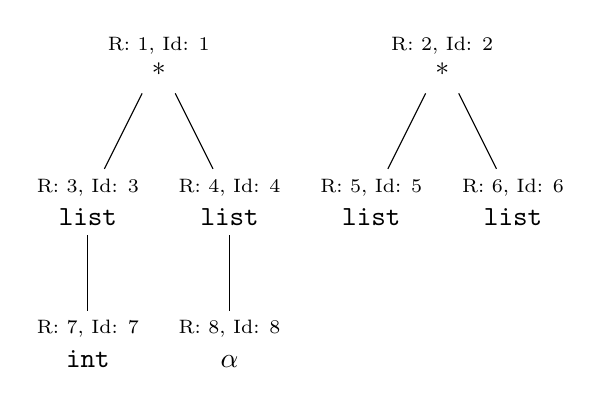
\begin{tikzpicture}
	[
		scale=0.90,
		N/.style = {rectangle, align=center, draw=none, fill=none},
		T/.style = {rectangle, align=center, draw=none, fill=none},
	]

	% times symbols
	\node[N] (*1) 	at ( 0.0, 4.0 ) {{\scriptsize R: 1, Id: 1}\\*};
	\node[N] (*2) 	at ( 4.0, 4.0 ) {{\scriptsize R: 2, Id: 2}\\*};

	% list symbols
	\node[N] (l1) 	at (-1.0, 2.0 ) {{\scriptsize R: 3, Id: 3}\\{\tt list}};
	\node[N] (l2) 	at ( 1.0, 2.0 ) {{\scriptsize R: 4, Id: 4}\\{\tt list}};

	% terminal symbols
	\node[T] (t3) 	at ( 3.0, 2.0 ) {{\scriptsize R: 5, Id: 5}\\{\tt list}};
	\node[T] (t4) 	at ( 5.0, 2.0 ) {{\scriptsize R: 6, Id: 6}\\{\tt list}};
	\node[T] (t1) 	at (-1.0, 0.0 ) {{\scriptsize R: 7, Id: 7}\\{\tt int}};
	\node[T] (t2) 	at ( 1.0, 0.0 ) {{\scriptsize R: 8, Id: 8}\\$\alpha$};

	\foreach \from/\to in {*1/l1,*1/l2,*2/t3,*2/t4,l1/t1,l2/t2}
	\draw[solid] (\from) -- (\to);

	\end{tikzpicture}
	\label{fig:mgu-algorithm-initial}
	\caption{Initial MGU {\tt list(int)*list($\alpha$)} and
	{\tt $\alpha$ * $\beta$}}
\end{figure}

\vfill\columnbreak

\begin{figure}[H]
	\center

	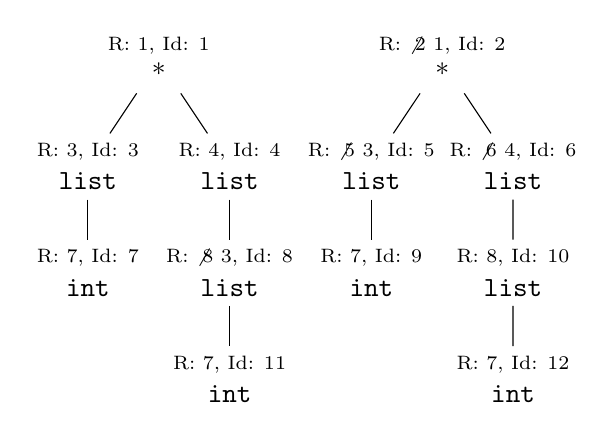
\begin{tikzpicture}
	[
		scale=0.90,
		N/.style = {rectangle, align=center, draw=none, fill=none},
		T/.style = {rectangle, align=center, draw=none, fill=none},
	]

	% times symbols
	\node[N] (*1) 	at ( 0.0, 3.0 ) {{\scriptsize R: 1, Id: 1}\\*};
	\node[N] (*2) 	at ( 4.0, 3.0 ) {{\scriptsize R: $\not2$ 1, Id: 2}\\*};

	% list symbols
	\node[N] (l1) 	at (-1.0, 1.5 ) {{\scriptsize R: 3, Id: 3}\\{\tt list}};
	\node[N] (l2) 	at ( 1.0, 1.5 ) {{\scriptsize R: 4, Id: 4}\\{\tt list}};

	% terminal symbols
	\node[T] (t3) 	at ( 3.0, 1.5 ) {{\scriptsize R: $\not5$ 3, Id: 5}\\{\tt list}};
	\node[T] (t4) 	at ( 5.0, 1.5 ) {{\scriptsize R: $\not6$ 4, Id: 6}\\{\tt list}};
	\node[T] (t1) 	at (-1.0, 0.0 ) {{\scriptsize R: 7, Id: 7}\\{\tt int}};
	\node[T] (t2) 	at ( 1.0, 0.0 ) {{\scriptsize R: $\not8$ 3, Id: 8}\\{\tt list}};
	\node[T] (t5) 	at ( 3.0, 0.0 ) {{\scriptsize R: 7, Id: 9}\\{\tt int}};
	\node[T] (t6) 	at ( 5.0, 0.0 ) {{\scriptsize R: 8, Id: 10}\\{\tt list}};
	\node[T] (t7) 	at ( 5.0,-1.5 ) {{\scriptsize R: 7, Id: 12}\\{\tt int}};
	\node[T] (t8) 	at ( 1.0,-1.5 ) {{\scriptsize R: 7, Id: 11}\\{\tt int}};

	\foreach \from/\to in {*1/l1,*1/l2,*2/t3,*2/t4,l1/t1,l2/t2,t3/t5,t4/t6,t6/t7,t2/t8}
	\draw[solid] (\from) -- (\to);

	\end{tikzpicture}
	\label{fig:mgu-algorithm-applied}
	\caption{Applied MGU {\tt list(int)*list($\alpha$)} and
	{\tt $\alpha$ * $\beta$}}
\end{figure}

\end{multicols}

By the most-general unifier algorithm we then get that the unified types of
$\alpha$ and $\beta$ are
\begin{align*}
	\alpha &\rightarrow {\tt list(int)} \\
	\beta &\rightarrow {\tt list(\alpha)} \rightarrow {\tt list(list(int))}
\end{align*}
From this these deductions we have that the unified type is {\tt list(int) *
list(list(int))}.

% Note that each type variable, i.e., greek letter, appears only once in the
% unification graph,albeit it can be the destination of many edges. For
% example, there is only one alpha node reachable via both type expressions.
% (This property is assumed by the unification algorithm!)

\end{document}
